\section{Diskussion}
\label{sec:Diskussion}

In der Auswertung kam es bereits zu einigen unrealistischen und offensichtlichen
falschen Werten die alle aus Berechnungen stammten.
Im Folgenden soll die Ursache für die dramastischen Abweichungen analysiert werden.


Dafür soll zu Beginn die Messung an sich überprüft werden.
Dazu wird die jeweilige theoretische Schwingungsdauer mit den gemessenen Schwingungsdauern verglichen.
\begin{figure}
    \centering
    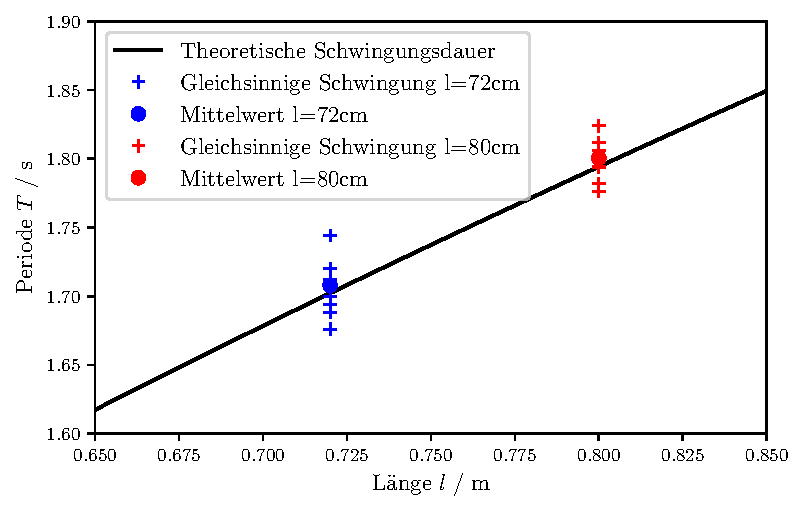
\includegraphics[width=0.5\textwidth]{plots/plot1.pdf}
    \caption{Gleichsinnige Schwingungen}
\end{figure}
Die Theoretische Kurve folgt aus Glichung (6!). Es wird deutlich, dass die gemessenen
Schwingungsdauern $T_+$ mit den zu erwartenen Schwingungsdauern übereinstimmt.\\

Für die gegensinnige Schwingung ergibt sich der zu erwartende theoretische Werte aus Geichung (8!).

\begin{figure}
    \begin{subfigure}[c]{0.5\textwidth}
        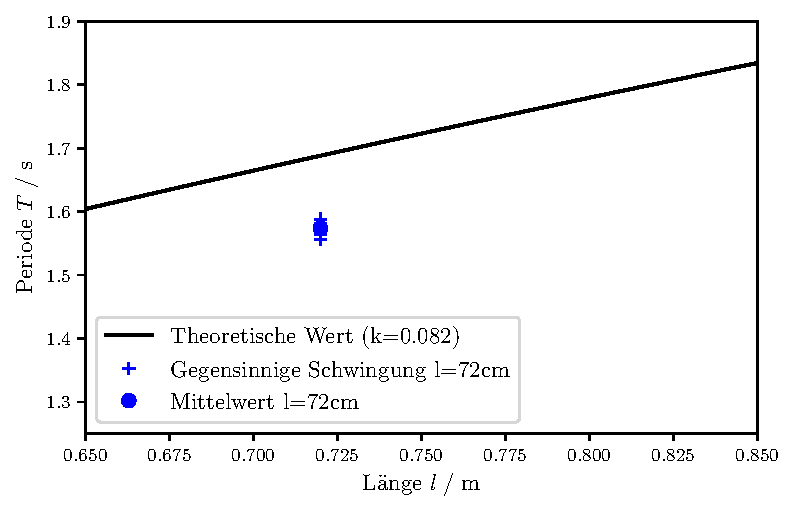
\includegraphics[width=\textwidth]{plots/plot2.pdf}
        \subcaption{Pedel 72cm}
    \end{subfigure}
    \begin{subfigure}[c]{0.5\textwidth}
        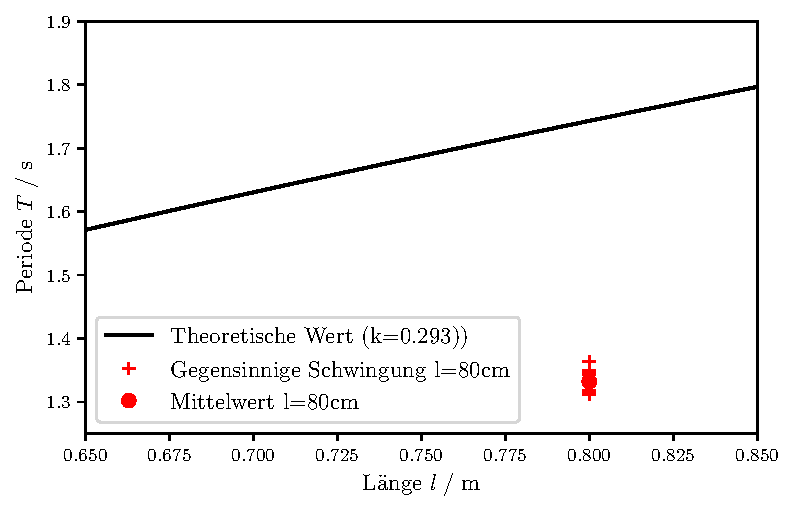
\includegraphics[width=\textwidth]{plots/plot3.pdf}
        \subcaption{Pendel 80cm}
        \label{fig:pedel80}
    \end{subfigure}
    \caption{Gegensinnige Schwingungsdauer}
\end{figure}

Hier bei wird besonders gut deutlich, dass bei \ref{fig:pendel80}, große Abweichungen
vorliegen. Dies lässt sich nur auf einen Messfehler zurückführen.
Weiterführend sei zu beachten, dass die Kopplungskonstante die für die theoretische Kurve
verwendet wird, ebenfalls aus diesen falschen Werten stammt.

Dies erklärt weiterführend, warum die Kopplungskonstant aus \ref{eqn:kopplung80} nicht die selben
sind.
Behauptung: Der Messfehler der Gegensinnigen Schwingung von der Pendellänge $l=80cm$ und $l=72cm$ ist 
ist ein Ursprung der Fehler.

Stellt man Gleichung (\ref{eqn:T_m}) um, um die Größenordung der Kopplungskonstante $K$ zu erörtern, so gilt:
\begin{equation}
    K=\frac{2\pi^2l}{T_{-}^2}-\frac{g}{2}
\end{equation}
Somit ergibt sich:
\begin{align*}
    \textrm{K für 72cm} = 0,833\\
    \textrm{K für 80cm} = 3,995 
\end{align*}
Für diese neuen Kopplungskonstanten sei gesagt, dass sie nur als Größenordnung diehnen.
Denn durch die passenden gleichsinnigen Schwingungsdauern $T_+$und den fehlerhaften gegensinnigen Schwingungsdauern $T_-$
folgt nach Gleichung (\ref{eqn:Kopplungkonstante}) eine fehlerhaft Kopplungkonstante $K$.
 
Trägt man für diese neuen Kopplungskonstanten die gegensinnigen Schwingungen auf, dies Bestätig die Annahme
das der Fehler in den gemessenen gegenphasigen Schwingungsdauern.  
\begin{figure}
    \begin{subfigure}[c]{0.5\textwidth}
        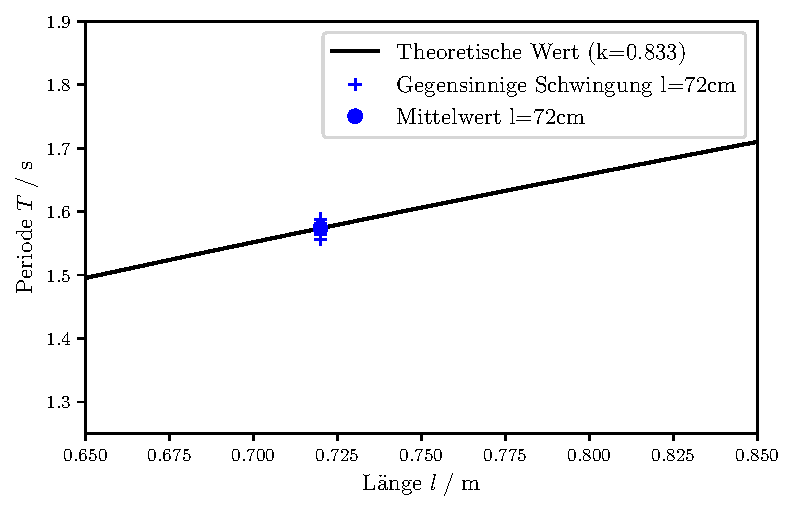
\includegraphics[width=\textwidth]{plots/plot4.pdf}
        \subcaption{Pedel 72cm}
    \end{subfigure}
    \begin{subfigure}[c]{0.5\textwidth}
        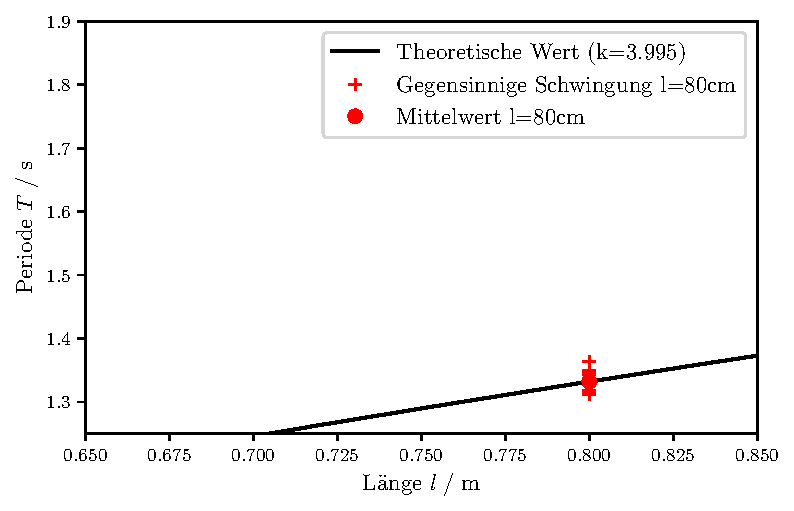
\includegraphics[width=\textwidth]{plots/plot5.pdf}
        \subcaption{Pendel 80cm}
        \label{subfig:gegenNEU80}
    \end{subfigure}
    \caption{Gegensinnige Schwingungsdauer mit Kopplungskonstante}
\end{figure}

Fazit: Der Fehler findet sich beim Messen der gegensinnigen Schwingungen und
zieht sich dann durch die Rechnungen für die berechneten Kopplungskonstante $K$ und die Frequenzen $\omega$
so wie für die Schwebungsdauer.\\
Somit stimmen gemessene und berechnete Werte nicht überein.


